
\Chapter{GAN teljesítmény mérés és regularizációs módszerek}

A gépi tanulásos modellek tanítási életciklusának utolsó lépése optimális esetben a tesztelés. Hagyományos esetben a dataset-et három részre osztjuk fel: Tanító-, teszt- és validáló halmazra. Hogy ezt milyen arányban tesszük meg, az függ a problémától is, de általánosan a teszt adathalmaz a dataset 20\%-a is lehet, a validáló halmaz még kissebb szelete a datasetnek és a tanítóhalmazon történik a modell tanítása.
A teszt halmazt csupán egyetlen egyszer láthatja hagyományos esetben a modell, a tanítás után.
A teszthalmazzal szimuláljuk a modell valós adatokra történő alkalmazását, hiszen a modell számára ezen adatok teljesen ismeretlenek lesznek. A tesztadatok az eredeti dataset elemei, így rendelkezésünkre állnak az elvárt eredmények is, így a modell predikcióit össze tudjuk vetni az elvárt kimenettel, amelyből megbecsülhetjük a modell pontosságát különféle metrikák szerint.
A GAN esetében osztályozási feladatot a diszkriminátor lát el, viszont a hamis adatok nem részei a datase-ünknek, azok a generátor által kreálódtak. A betanított modellnek csupán a generátora kerül felhasználásra, hiszen ezen komponens önmagában képes előállítani az új adatokat. A diszkriminátornak csupán a tanítás során van jelentősége és a validálásra önmagában nem alkalmas, hiszen ha a diszkriminátorunk rosszul tanult, úgy a generátorunk sem fog tudni a datasethez hasonló képeket generálni.
A GAN esetében nem szokás a datasetet feldarabolni tanító és teszt részre, hiszen nem tudjuk a generátorra alkalmazni a már ismert metrikákat.
Ha képek generálása a feladat, úgy még nehezebb dolgunk van, hiszen a képeken hordozott információ igen összetett lehet.
A generátor kiementét kell valamilyen módon tesztelnünk, ami nem egy egyértelmű feladat.
Egy emberi szemlélő természetesen meg tudná különböztetni a generált és a valós képeket. Lényegében a diszkriminátor feladatát látná el az emberi tesztelő, akinek hasonlóad mutathatnánk valódi és generált képeket, amelyekről el kell döntenie, hogy melyik a valódi és melyik a hamis. A fotorealisztikus képgenerálás igen nehéz feladat és ha egy kicsit is rosszul teljesít a modell, azt egy emberi szemlélő hamar észreveszi és a modell pontossága igen alacson lesz az emberi megfigyelő ítéletei alapján. Ha visszajelzést is kap az ember a hibáiról, akkor Salimas et al. megfigyelték, hogy a továbbiakban sokkal pesszimistább ítéletet hoznak a tesztelők a képekre. Bináris, osztályozás helyett diszkrét vagy folytonos skálán is mérhetnénk a generált képeink jóságát. A pontos mérési eredmények érdekében több résztvevőt is be kéne vonnunk a tesztelébe. Már belegondolva is igen lassú és költséges feladat lenne a modellünk tesztelése, így nem hagyatkozhatunk az emberi validálásra. Ez motiválta Salimas et al.-t is.

Az alábbi két ajánlás két mérőszámot definiál, amelyek segítségével meghatározhatjuk a GAN modellünk teljesítményét. Ezen validálási technikák megjelenése óta az újjonnan megjelent GAN architektúrák mindegyikét lemérték és a GAN-al foglalkozó cikkekben táblázatokban vetik össze a különféle modellek teljesítményét a sajátjukkal.
A két mérőszámot együttesen szokták alkalmazni, hiszen egyik módszer sem tökéletes, viszont a kettőt együtt alkalmazva ad egy bizonyos képet a modellünk teljesítményéről.
A két mérőszám közös jellemzője, hogy mindkettő az Inception modell által kinyert jellegvektorok alapján határozza meg a modell jóságát.

Az alábbi kódrészlet az ImageNet adathalmazon betanított Inception modell használatát kívánja szemléltetni a Keras segítségével. A kódrészlet első futtatásakor a modell súlyai letöltésre kerülnek és a további betöltés esetén egyből rendelkezésre fog állni.

\begin{python}
from tensorflow.keras.applications import InceptionV3

inception_model = InceptionV3(weights='imagenet')
predictions = inception_model.predict(images)
\end{python}

Az Inception modell bemenete alapértelmezett beállítasok mellett egy 299x299 -es felbontású rbg színcsatornákkal rendelkező kép. A pixelértékeket normalizáltan várja a modell a $[-1, 1]$ tartományon. A modell inicializálásakor paraméterként megadhatjuk a bemenet méretét, viszont az nem lehet 75x75-nél kisebb. Ha az \texttt{include\_top} paramétert \texttt{True} értékkel állítjuk be, úgy a modell tartalmazni fogja az utolsó Dense rétegét is, amely az ImageNet súlyok alapján betanított modell esetében 1000 osztály detektálására lesz képes.

Az említett, GAN teljesítménymérésére használatos módszerek az \textit{Inception Score} (IS) és \textit{Fréchet Inception Distance} (FID). Ezeket kívánom bemutatni az alábbi két alfejezetben.

\Section{Inception Score}
Az Inception Score \cite{salimans2016improved, barratt2018note} technikát Salimans et al. az emberi tesztelés automatizálására vetette fel. A méréseik alapján a technika sok minta figyelembevételével igen jól közelíti az emberi tesztelők által mért eredményeket.
Alapjául az Inception model szolgál, amelyet az ImageNet dataseten tanítottak be. Minden egyes generált képet beadnak inputként a betanított Inception modellnek, hogy megkapják a conditional label eloszlást $p(y|x)$. Az olyan képeken, amelyeken jelentőségteljes objektumok figyelhetők meg, alacsony entrópiájú $p(y|x)$-el kell rendelkeznie. Vagyis a generált képen minél kevesebb objektumot kell felismernie a modellnek.
Továbbá az is lényeges szempont, hogy a generátor különféle képeket generálon, így a következőnek magas entrópiával kell rendelkeznie:
$$ \int p(y|x = G(z))dz $$

Az Inception Score tehát:

$$ \exp(\mathbb{E}_x KL(p(y|x)||p(y))) $$

Minél magasabb ez a szám, annál jobb a GAN teljesítménye. Természetesen az IS is kijátszható és hamis eredményeket is adhat. (Note on IS-ben van róla szó)

TODO: Írni még erről gondolatokat, pontosítani

[Az inception score kódja]\\(https://github.com/openai/improved-gan/tree/master/inception\_score)
TODO: Inception score implementálása Tensorflow 2-ben? Vagy az eredetivel kéne mérni? (Az még tf1-es)


\Section{Fréchet Inception Distance}
Az Incepton Score kiegészítésére megjelent egy másik, széles körben elfogadott teljesítménymerő technika, a Fréchet Inception Distance (FID) \cite{heusel2017gans}. Az IS nem vette figyelembe a tanítóminta statisztikáit, és ez egy igen nagy hátránya a technikának. Továbbá az IS feltételein is javítottak, hogy a mintákon megtalálható zajok is befolyásolják a végső eredményt.

TODO: Pontosítás!!!

Minél alacsonyabb az FID, annál jobb a modell teljesítménye az adott tanítómintán.

TODO: Összefoglaló táblázat, saját modellek eredményei, ábrák




\Section{Mode collapse jelenség}

A Mode collapse jelenség alatt a tanulás során bekövetkező anomáliát értjük, amely hatására a Generátor a látens tér bármely pontjára ugyanolyan kimeneti képet generál. A képek között minimális változatosság ugyan megfigyelhető, ugyanakkor az is látható, hogy a képeken igen hasonló formák jelennek meg.

Ez a jelenség valójában tekinthető egyfajta overfitting-nek is, vagyis túltanulásnak. Viszont a mode-collapse elnevezés találóbb, hiszen amikor ez bekövetkezik, akkor a további tanítási lépések során úgy tűnhet, hogy stablian tűnő modell hirtelen összeomlott volna.
A mode-collapse fellépése esetén a model további tanítása során minden egyes epoch-al változik a mode, vagyis az előzőtől eltérő kép jelenik meg a kimeneten (szintén minden egyes mintavételezett pontra hasonló). Mivel a diszkriminátor a mini-batch minden egyes bemenetét egymástól függetlenül dolgozza fel, így a gradienseiben sem jelenik meg olyan információ, amely a generátort változatosabb képek generálására bíztatná. A mode collapse esetén a diszkriminátor egyetlen pontot képes csak valódi adatnak tekinteni, majd minden egyes frissítéssel a pont elmozdul, ezzel magyarázható, hogy az összeomlás után tanítva minden egyes iterációval változik ezen pont, amire \textit{mode}-ként szokás hivatkozni \cite{salimans2016improved} Vagyis a GAN modellünk használhatatlanná válik.

"Helvetica scenario"

\begin{figure}[h]
\centering
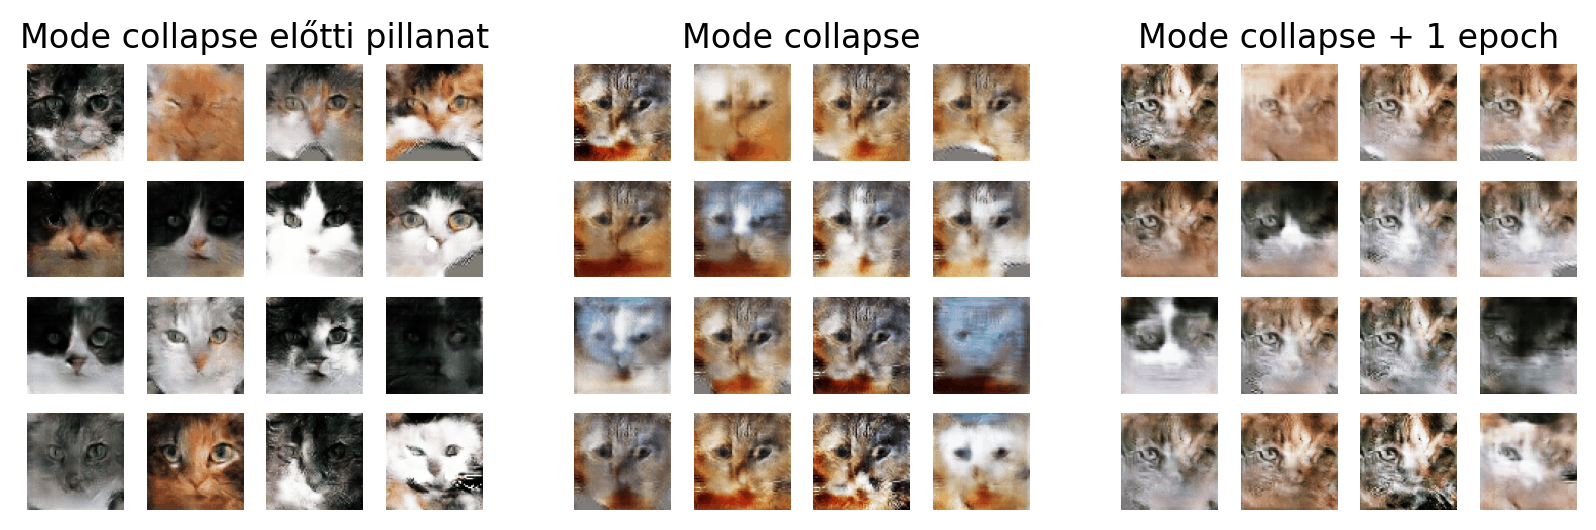
\includegraphics[width=15cm]{images/mode-collapse.png}
\caption{Mode collapse jelensége}
\label{fig:mode-collapse}
\end{figure}

A tanítás közben felléphetnek lokális mode-collapse-ok is, amelyek a látens-tér egyes tartományaiban alakulhat ki (Stackgan2-ben vizsgálták ezt).

Egyes cikkekben az összeomlásig tanítják a felvázolt modelleket és az összeomlás előtti állapotokra állítják vissza a hálózat súlyait a használathoz \cite{brock2018large}

TODO: Mode collapse okok pontosabb leírása, detektálási technikák megnézése

A GAN tanítása során nehézségekbe ütközhetünk. Legrosszabb esetben nem is kezd el konvergálni a generátor kimenete a tanítóminta képeihez, viszont abban az esetben gyanakodhatunk, hogy a modellünk nem lett helyesen felépítve. Amennyiben mégis elkezd fejlődni a modell és nem csak zaj jelenik meg a kimeneten az egyes tanítólépések után, de bizonyos számú epoch után mode collapse lép fel, úgy fontolóra vehetjük a következő regularizációs technikákat.

\Section{Regularizációs módszerek}
\SubSection{Label-smoothing}
A label-smoothing az egyik legegyszerűbb regularizációs trükk, amely a neurális hálók overfitting problémáját kívánja kiküszöbölni. Ezen módszer alkalmazásához nem szükséges módosítanunk az architektúránkat, csupán a hibafüggvényt, így ez egy egészen egyszerűen implementálható technika. GAN esetében a diszkriminátor hibafüggvényét szokás módosítani oly módon, hogy a bináris keresztentrópia számolás során a valós bemeneti képek 1-es címke helyett valamennyivel alacsonyabb értéket, például 0.9-et kapnak. Ezzel a beállítással a diszkriminátor kevésbé lesz hajlamos a túlzott magabiztosságra a valós bemeneti képek esetén, teret adva a generátor fejlődésének.

A regularizációs technikákban megfigyelhető néhány esetben egy kicsi ellentmondásosság is, például egyes technikák a diszkriminátort hátráltatják, míg mások a generátor dolgát nehezítik meg. Természetesen a problémától függ, hogy melyik módszer alkalmazható egy adott modellnél.

\begin{python}
def discriminator_loss(real_output, fake_output):
    real_loss = cross_entropy(
        tf.constant(np.full(fake_output.shape, 0.9)),
        real_output)
    fake_loss = cross_entropy(
        tf.constant(np.full(fake_output.shape, 0)),
        fake_output)
    total_loss = real_loss + fake_loss
    return total_loss
\end{python}

\SubSection{Megfelelő inicializációs stratégia}

A mély neurális hálózatoknál igen gyakran előforduló probléma az úgynevezett exploding vagy éppen a vanishing gradiensek jelensége, amelyet gyakran csupán instabil gradienseknek is szokás nevezni.
A tanítás forward-propagation stádiumában a hálózat kimenetén megfigyelhető túl magas vagy éppen túl alacsony értékek a hibafüggvény meghatározásánál is szélsőséges értékeket okozhatnak.
A backpropagation stádiumában az output rétegtől haladunk az input felé, amely során kiszámolásra kerülnek a gradiensek a hálózat minden egyes paraméterének függvényében. Majd Gradient Descent vagy ahhoz hasonló algoritmus segítségével frissülnek a hálózat paraméterei. Mindkét irányban fontos lenne elkerülni az esetleges kilengéseket, hogy a tanítás stabilitását elősegítsük.
Az olyan hálózatoknál, amelyekben több rejtett réteg is található, az instabil gradiensek jelensége még inkább érvényesül. A backpropagation során az input réteg felé haladva a gradiensek hajlamosak lehetnek igen kis értékekre zsugorodni. Ilyen esetben az alacsonyabb rétegek rendszerint lassabban fognak tanulni, amely szintén komoly problémát jelent.
A hálózat rétegeiben megtalálható neuronok az előző rétegek neuronjaitól függenek, illetve a kimenetük a következő réteg neuronjait is befolyásolja. Egy esetlegesen fellépő túl magas vagy túl alacsony kilengés a kimeneti értékekben komoly hatással lehet a teljes hálózatra.

Az instabil gradiensek megelőzésére az egyik irány a neuronok inicializációs stratégiájának megválasztása.
Az évek során több ajánlás is érkezett, a különböző felépítésű hálózatokra különböző technikák váltak be.

Kiemelnék két inicializációs technikát, a Glorot \cite{glorot2010understanding} és a He \cite{he2015delving} stratégiákat, amelyek széleskörűen alkalmazhatónak bizonyultak.
A kezdőértékek generálásához figyelembe veszik a rétegek be- és kimeneti kapcsolatainak számát is, amelyet $fan_{in}$ és $fan_{out}$-nak is nevezhetünk és azok átlagát használják fel a számoláshoz.

$$fan_{avg} = \frac{fan_{in} + fan_{out}}{2}$$

A \textbf{Glorot/Xavier} inicializációs stratégia normális és egyenletes eloszlásra is számolható.
Normális eloszlás esetén a várható értéket $m = 0$-ra kell választani, a szórásnégyzet pedig: $ \sigma^2 = \frac{1}{fan_{avg}} $.

$$ \mathcal{N}(0, \frac{1}{fan_{avg}}) $$

Egyenletes eloszlás esetén $\pm r$ között,

$$r = \sqrt{\frac{3}{fan_{avg}}}$$

$$ \mathcal{U}\left[-r, r\right] $$

Ezen inicializációs stratégia a tangens-hiperbolikusz, logisztikus és szoftmax aktivációs függvényekkel rendelkező rétegekben használatosak. 

A \textbf{He/Kaiming} inicializáció hasonló megközelítést alkalmaz,
Normális eloszlásra:

$$ \mathcal{N}(0, \frac{2}{fan_{in}}) $$

Egyenletes eloszlásra:

$$r = \sqrt{3\frac{2}{fan_{in}}}$$

$$ \mathcal{U}\left[-r, r\right] $$

Ezen inicializációs stratégia pedig a ReLU aktivációs függvénnyek családjával rendelkező rétegekben ajánlott használni.

A Keras a Glorot inicializálást használja alapértelmezetten.

TODO: Egyszerű példákkal szemléltetve az eredményeket.


\SubSection{Batch Normalization}
Az instabil gradiensek problémája a tanítás során is jelentkezhet, a megfelelő inicializációs stratégia nem garantálja a teljes stabilitást, csupán egy kezdeti optimális állapotot biztosít a modellnek.
Az input adatok standardizálása áll a Batch Normalization technika mögött, amelyet a rétegek között vagy a rétegek aktivációs függvénye előtt ajánlott megtenni. A Batch Normalization technika alkalmazásához tehát minimálisan módosítanunk kell a meglévő modelljeink architektúráját. Viszont úgy figyeltem meg, hogy ezen technika alkalmazása teljesen empirikus módon történik és nincsen egy általánosan elfogadott módszer arra sem, hogy pontosan hol kell elhelyezni a réteget (az aktivációs függvények előtt vagy után vagy mindkét helyen bigGAN esetében mindenhova rakták, a többit meg kell néznem). A GAN esetében a kezdeti próbálkozásban csupán a diszkriminátorban (tényleg így van?) helyezték el a rétegeket (melyik cikkekben láttam ezt?), majd a generátorban is alkalmazásra került. Kétségtelen, hogy a technika alkalmazásával stabilabb tanítást eredményez és széleskörűen alkalmazható a mély neurális hálózatokban.

A Batch Normalization technika zero-centerezi és normalizálja az inputokat, majd skálázza és shifteli az eredményeket. Vagyis két tanulható paramétervektor jelenik meg rétegenként a modellünkben, a skálázásra és shiftelés műveletre. A technika neve a mini-batch tanítási stratégiából adódik, vagyis amikor egy tanítási lépést nem a teljes dataset-re hajtunk végre, csupán egy annak kisebb szeletére. A Batch Normalization zero-centerező és normalizáló lépéséhez az algoritmusnak meg kell becsülnie az aktuális bemeneti mini-batch várható értékét és szórását. Ezt a becslést csupán tanítási időben tudja megtenni az algoritmus, hiszen olyankor rendelkezésére áll a teljes mini-batch. Viszont tesztelésnél, amikor csupán egy-egy tesztadatot lát a modell, úgy nem hagyatkozhatunk a becsült várhatóértékre és szórásra. A Keras-ban található implementáció a tanulás során mozgóátlaggal vezeti a várhatóértékeket és a szórásokat. Ez további két paramétert jelent, amelyeket a modell a tanulási folyamat során fog meghatározni a már említett módon, viszont a backpropagation során nem kerülnek finomhangolásra, csupán tesztidőben kerülnek felhasználásra ezek az értékek.

Az algoritmus működése a következőképpen írható fel \cite{geron2019hands}:

Legyen $m$ a minibatch elemszáma $m \in \mathbb{N}, 0 > m \ge n$, ahol $n$ a dataset elemszáma

$m = \{x_1, x_2, \ldots, x_m \}$ 

1. Határozzuk meg a várható értékeket a mini-batch elemeire
$$ \vec{\mu} = \frac{1}{m} \sum_{i=1}^{m} x_i $$

2. Határozzuk meg a szórásnégyzeteket a minibatch elemeire
$$ \sigma^2 = \frac{1}{m} \sum_{i=1}^{m} (x_i - \mu)^2 $$

3. Zero-centerezzük és normalizáljuk az inputokat. $\varepsilon$ egy kicsi szám (általában $10^{-5}$), ami a 0-val való osztás elkerülése érdekében van jelen
$$ \hat{x_i} = \frac{x_i - \mu}{\sqrt{\sigma^2 + \varepsilon}} $$

4. Skálázzuk a $\gamma$ és shifteljük $\beta$ paraméterekkel az inputokat
$$ z_i = \gamma \otimes \hat{x_i} + \beta$$

Az algoritmus kimenete a $z_i$.

(sok GAN architektúrában megfigyelhető (melyek azok?) de pl a ProGAN ehelyett Pixelwise-normalization-t használ a generátorban)

\SubSection{Spectral Normalization}
\cite{miyato2018spectral}
(Ennek használata megengedi a nagyobb minibatch-méret használatát, hogy minél változatosabb képeket tudjon generálni a generátor. ennek utána kell néznem, hogy pontosan hogyan működik)

- Lipschitz constant az egyetlen hyper-paraméter
- Egyszerű implementáció

While input based regularizations allow for relatively easy formulations based on samples, they also
suffer from the fact that, they cannot impose regularization on the space outside of the supports of
the generator and data distributions without introducing somewhat heuristic means.


$$ \sigma(A) := \max_{\boldsymbol{h}:\boldsymbol{h}\neq 0} \frac{\|A\boldsymbol{h}\|_2}{\|\boldsymbol{h}\|} = \max_{\|\boldsymbol{h}\|_2 \leq 1} \|A\boldsymbol{h}\|_2$$

A Spectral Normalization normalizálja a $W$ súlymátrix spectral normálisát oly módon, hogy az kielégítse a Lipschitz megkötést $\sigma(W) = 1$.



Lipschitz megkötés 3 módon:

Wasserstein GAN -> a critic-nek 1 folytonos Lipschitz térhez kellett tartoznia
Cliping the weights
Gradient penalty és a spectral norm

Optimális diszkriminátor: pdata(x)/(pdata(x)+Pg(x)

TODO: Pontosítani a SN-t!!!

\SubSection{Experience replay}
(A tanulás során a korábbi kimenetek egy bufferben való tárolása és időközönként a modellnek újra megmutatjuk az eredményeket. Biológiai ok: alvás és álmodás fontossága. A régi megtanult feature-ök megőrzését segíti elő)

\SubSection{Mini-batch discrimination}
A mode collapse jelenség egyik ismertetőjegye amikor a generáto kimenetén közel azonos képek figyelhetők meg. A diszkriminátor minden inputját függetlenül vizsgálja, így a tanulás során lényegében nem használja ki azt a lehetőséget, hogy mini-batch-okon tanítjuk. A már említett Batch-Normalization technika természetesen nem működne független bemenetekre, viszont a diszkriminátor döntése nem függ az egyidőben beadott inputoktól. Így a diszkriminátor az érkező mode collapse pillanatát nem képes érzékelni.
Erre a problémára kíván javaslatot tenni a Mini-batch discrimination technika, amelynek alapötlete az, hogy a diszkriminátor a döntéseit több bemenet kombinációiból határozza meg.
A cikkben felvetett implementációja az egymáshoz közeli képek detektálására irányul. Ha az inputként kapott mini-batch képei közel állnak egymáshoz, akkor az egész mini-batch-ot hamis címkével kell ellátni. Ezáltal az összeomlás egészen jól detektálható és ezen technika arra kényszeríti a generátort, hogy minél változatosabb képeket generáljon a hibafüggvényének minimalizálása érdekében.

A diszkriminátor egy belső rétegének kimenete egy transzfromáló tensoron keresztül mátrixokat alkot és ezeknek nézi meg a L1 normáját...


????? Zavaros !!!!!!!!

a belső feature-öket így jelöli: $f(x_i) \in \mathbb{R}^A $

a $T \in \mathbb{R}^{A \times B \times C} $

amiből lesznek mátrixok $M_i \in \mathbb{R}^{B \times C}$

$$ c_b(x_i, x_j) = \exp(- \|M_{i,b} - M_{j,b}\|_{L_1}) \in \mathbb{R} $$

L1 norma - Minél kisebb annál hasonlóbbak az inputok
Ez utána a következő réteg bemeneteként bemegy és ezek alapján változik meg a diszkriminátor

De a cikkben a feature matching-et jobbnak találták, viszont a későbbiekben pl a progan is használta a minimatch-ot??

\SubSection{Two Time-Scale Update Rule (TTUR)}
Ezen technikát szintén meg lehet valósítani architektúrális változtatás nélkül, csupán az Adam optimalizáló eljárás egyik paraméterét kell megfelelően beállítani az implementációjához.
Heusel et al. \cite{heusel2017gans} cikkjében mérésekkel alátámaztották, hogy ha az Adam optimalizáló módszert választjuk a GAN tanításához és a learning rate paramétert a generatároban és a diszkriminátorban különbözőre állítjuk, úgy a modell gyorsabban és stabilabban fog konvergálni a lokális optimumokhoz.

0.0001

0.0004

(különböző learning rate a generátorban és a diszkriminátorban)


